\section{\lr{CF\underline{ }ALS}}

\subsection{توضیحات کلی}

در این قسمت، روشی مانند روش 
\lr{Collaborative Filtering}
به کمک الگوریتم 
ALS
پیاده‌سازی شده است. ابتدا برای هر دوربین و هر ساعت از هفته، تعداد ترددها را به دست آوردم. سپس 
داده را به دو قسمت آموزش و آزمون تقسیم کردم. با کمک داده‌های آموزش مدل 
ALS
را 
train
کردم. سپس با کمک داده‌های آزمون دقت مدل خود را سنجیدم. 

مدل ما قابلیت این را دارد که به عنوان یک 
\lr{Recommender System}
عمل کند. در واقع می‌تواند برای هر دوربین و هر ساعت از هفته، تخمین بزند که چند 
ماشین در دوربین ثبت می‌شوند. کاربرد‌های آن می‌تواند به این صورت باشد که به ما کمک 
کند تصمیم بگیریم آیا یک دوربین در یک زمان خاص نیاز است روشن باشد یا خیر (مثلا 
ممکن است بتوانیم بسیاری از دوربین‌ها را فقط برای چند روز خاص به کار 
بگیریم). 
ممکن است یک دوربین در چند روز ترافیک شدیدی را ثبت کند، در این صورت می‌توانیم 
الگوریتم‌هایی پیش‌نهاد دهیم که به کمک این داده، برای روز‌های بعد مسیر‌های جایگزینی 
به راننده‌ها پیشنهاد دهد. 


\subsection{نتایج}

برای آزمایش مدل خود، علاوه بر توابع آماده که در کد دیده‌ می‌شود، چند دوربین به 
دلخواه انتخاب کردم و داده‌های آنان که در قسمت تست قرار داشت را در نظر گرفتم. 
دقت کنید که مدل ما هیچ وقت این داده‌ها را ندیده‌ است. سپس مقادیر واقعی این داده‌ها 
و مقادیر پیش‌بینی شده را با هم بر روی نمودار نشان دادم. یعنی برای برخی ساعات از روز 
حدس زدم که یک دوربین خاص، احتمالا چند ماشین ثبت می‌کند و 
آن را با مقدار واقعی مقایسه کردم. خطوط قرمز برای داده‌های واقعی و خطوط سیاه مقادیر پیش‌بینی شده هستند. همانطوری که می‌بینید دقت مدل تا حد قابل قبولی بالا است.

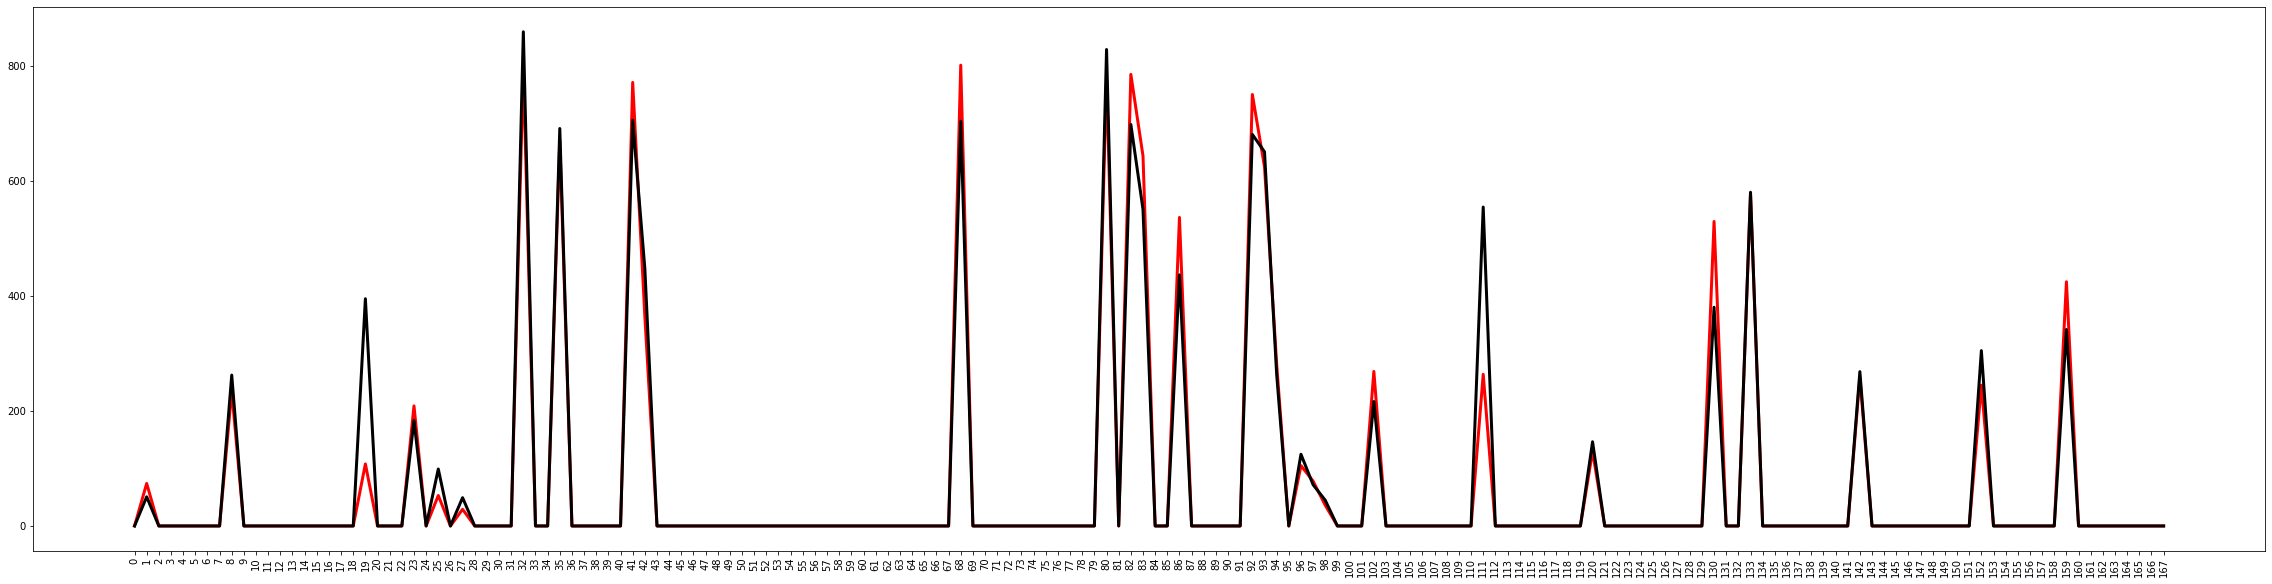
\includegraphics[scale=0.2]{images/CF_ALS/100.png}

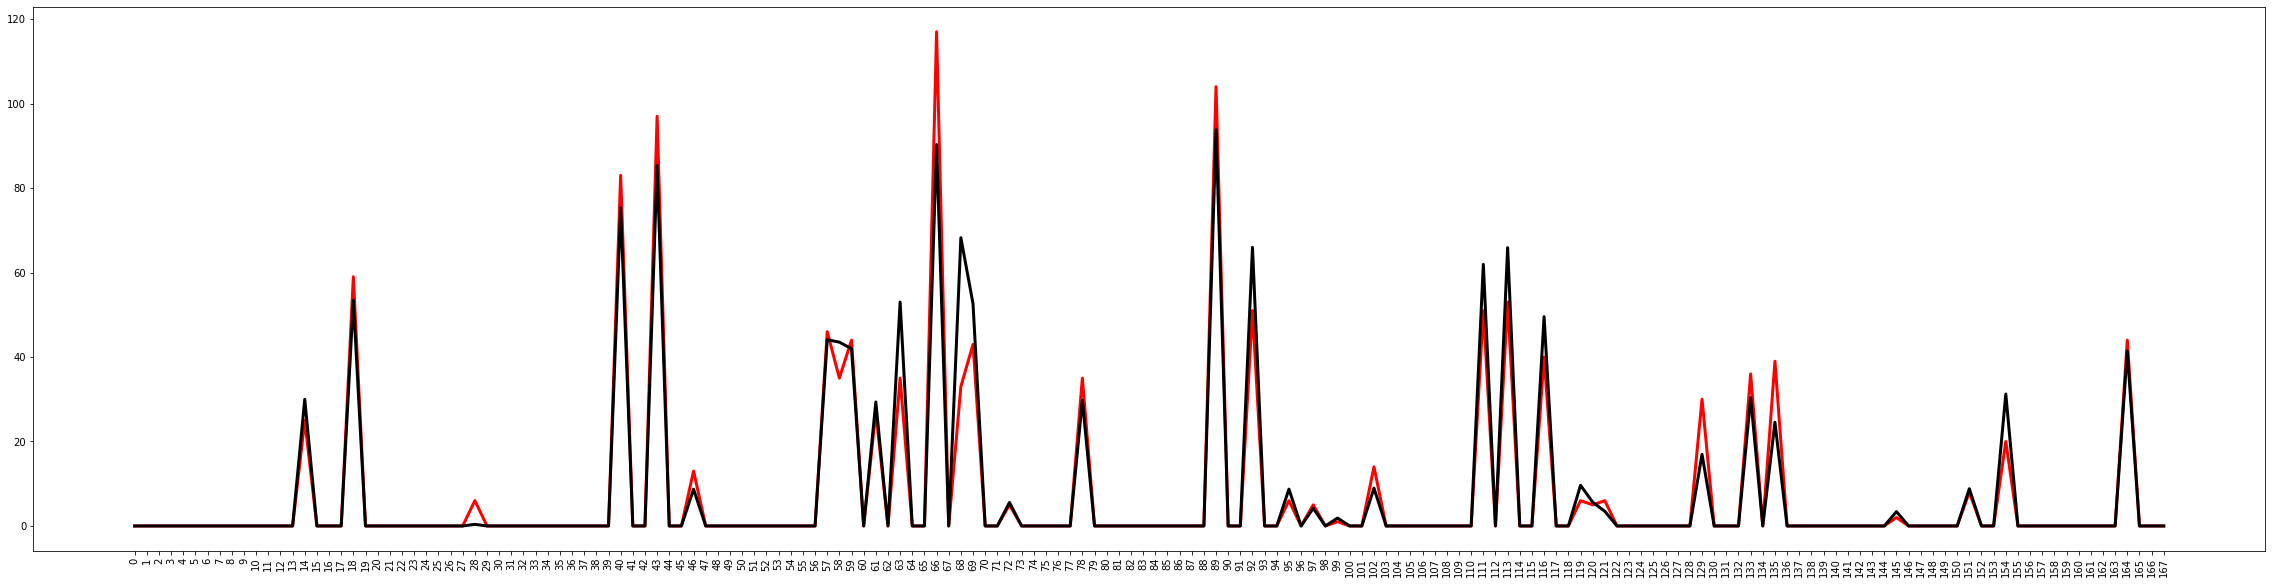
\includegraphics[scale=0.2]{images/CF_ALS/101.png}

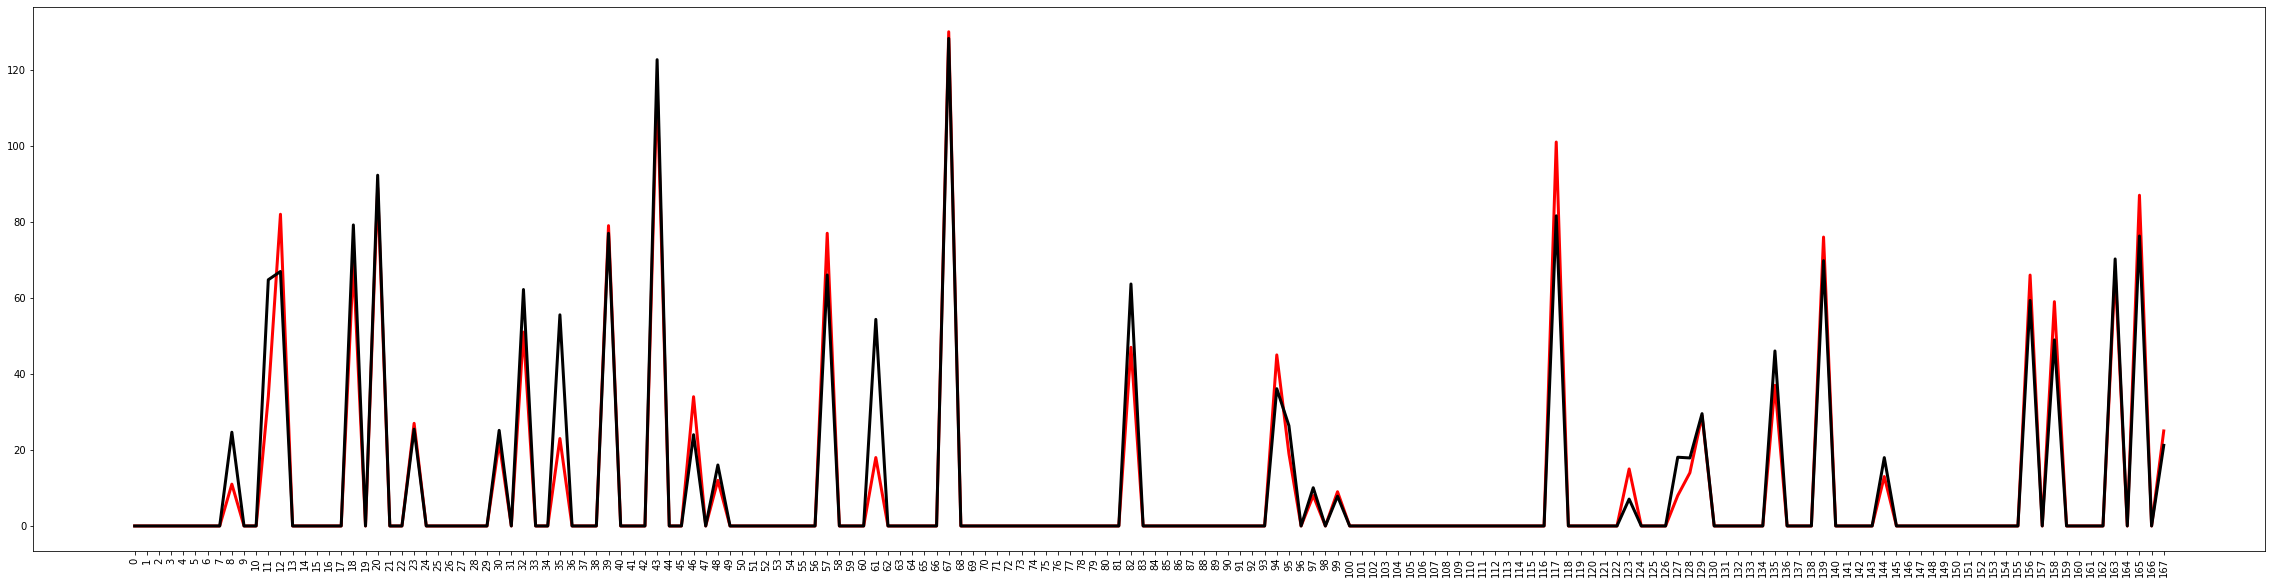
\includegraphics[scale=0.2]{images/CF_ALS/102.png}

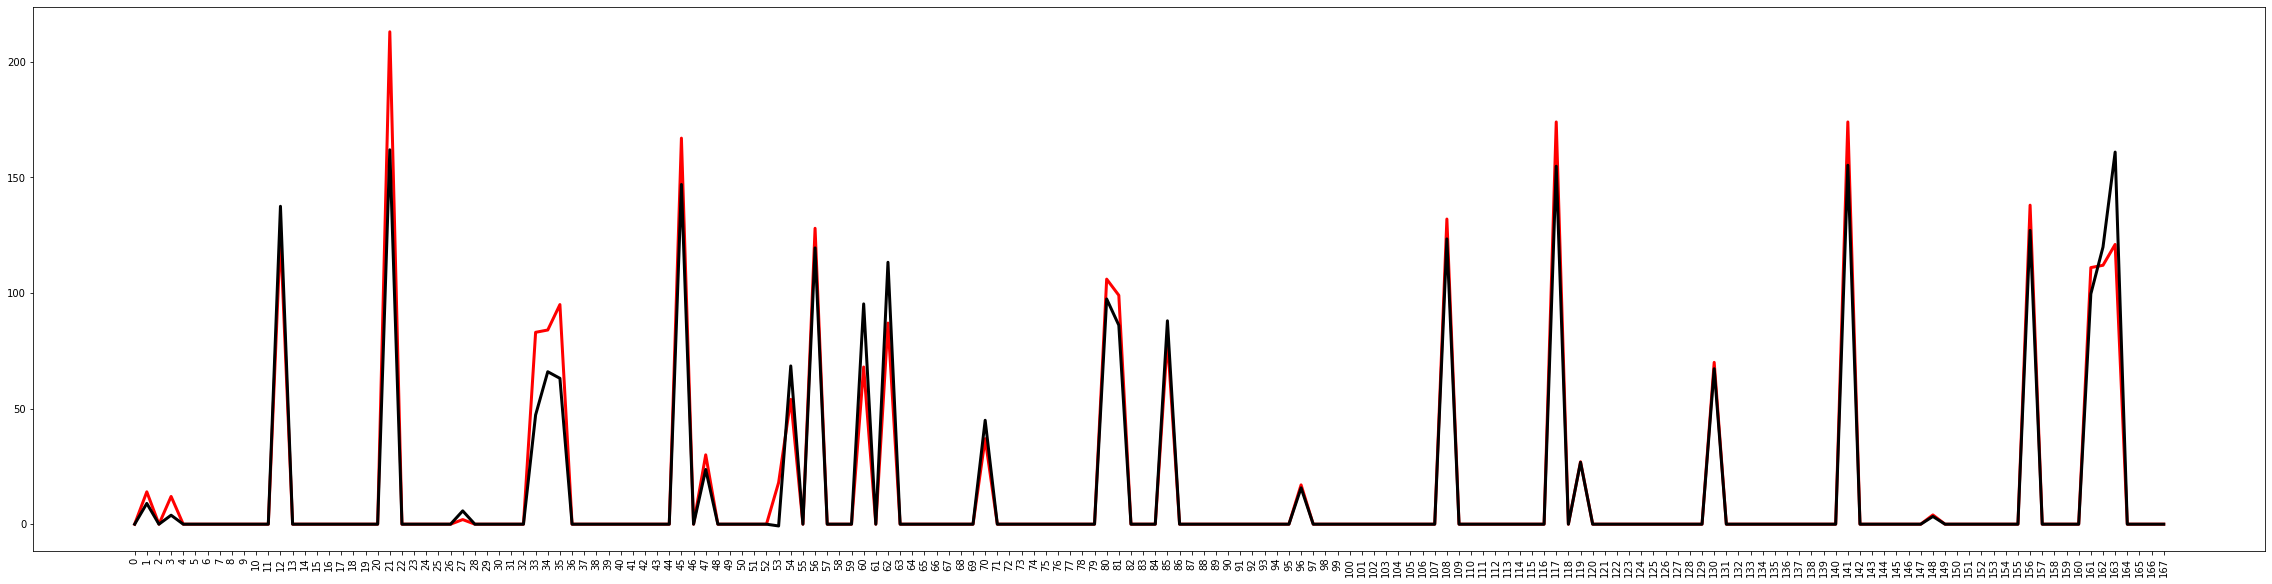
\includegraphics[scale=0.2]{images/CF_ALS/103.png}

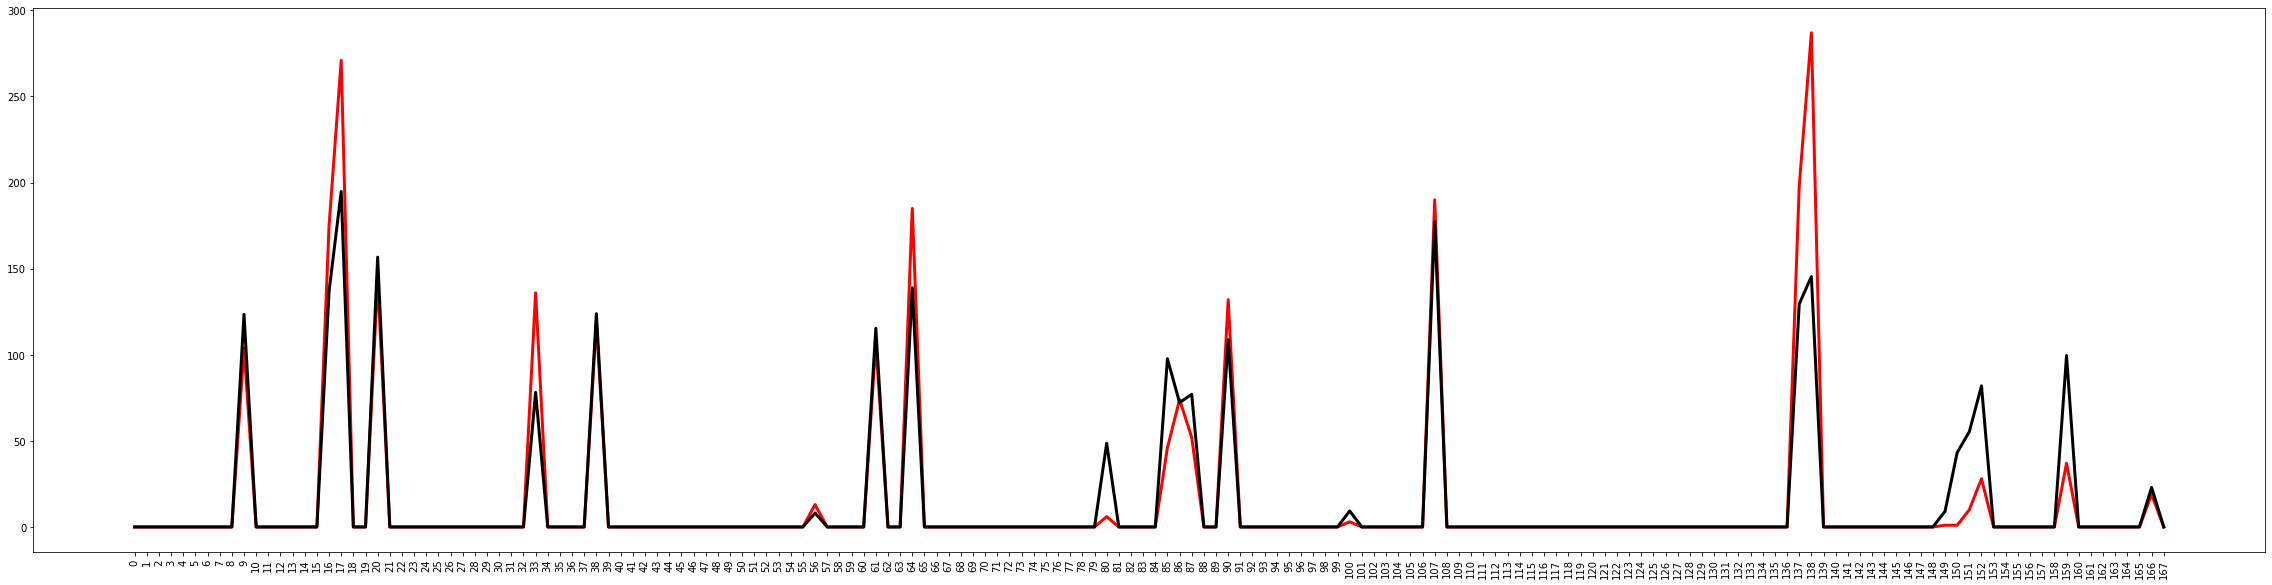
\includegraphics[scale=0.2]{images/CF_ALS/104.png}
